\documentclass[UTF8]{ctexart}
\usepackage{graphicx}
\usepackage{amsmath}
\usepackage{cite}
\usepackage{mathtools}
\usepackage[a4paper,left=2.5cm,right=2.5cm,top=3cm,bottom=3cm]{geometry}
\title{RGB配色实验:实验报告}
\author{禤科材 PB20030874 20级14系 707组 1号台}
\date{\today}
\bibliographystyle{plain}
\begin{document}
    \maketitle

   \section{实验目的}
   \begin{center}

    (2)理解LED灯原理与特性

    (3)掌握色光相加混色规律
   \end{center}
   
    \section{实验原理}
    \begin{center}
        \emph{\zihao{-4}自然界的三基色}\\[0.4cm]
    \end{center}

    自然界中人眼所能观察到的绝大多数颜色,都可以由三种相互独立的基本颜色按一定的比例混合
得到;相反,自然界中的任意一种颜色又可以被分解为不同比例的相互独立的三种基色,即三基色是颜色空间的一组基。
三基色之间的比例,直接决定混合色的色调和色饱和度,混合比例相同时,色调是相同的。
通过改变三束光的的强度,可以得到不同颜色的彩色光。

\begin{center}
    \emph{\zihao{-4}发光二极管}\\[0.4cm]
\end{center}

发光二极管,简称 LED,是一种直接将光能转化为电能的半导体器件。LED 是由$III$-$V$族化合物半导体
材料构成,其核心是 PN 结。它具有一般 PN 结的正向导通,反向截止、击穿特性。
在正向电压下,电子由 N 区注入 P 区,空穴由 P 区注入 N 区,从而结区出现不平
衡状态,这些注入的的电子与空穴在 PN 结区发生复合,发射光子。

理论和实践证明,发射光子的能量与材料能隙有下面的关系式:

\begin{equation}
    \lambda =\frac{1240}{E_g}(nm)
\end{equation}

式中,$E_g$的单位为电子伏特(eV)。因不同的材料,电子和空穴所占的能级也有所不同,能级差影响
电子和空穴复合后发射光子的能量,从而产生不同波长的光。若能产生可见光(380~760 nm),半
导体材料的$E_g$应在 3.26~1.63 eV 之间。
当加在二极管两端的电压接近导通阈值电压$U_D$时,二极管电流将会迅速增大,此后电流再增大,电压几乎不变,阈值电压$U_D$与禁带宽度$E_g$有下列关系:
\begin{equation}
    U_D=\frac{E_g}{e}
\end{equation}

其中$e$是元电荷电量,$U_D$在伏安特性曲线图上取得,通过式(1)与式(2)可以计算得知发光二极管的发光波长。

    \section{实验步骤}

    \emph{\\[0.02cm]\zihao{-4}1.测量LED的伏安特性曲线与发光波长}

    如图接线,在$0mA$至$100mA$内,分别测量红、绿、蓝 LED 的正向电压与电流关系,
    绘制红、绿、蓝 LED 的$U-I$特性曲线,并基于伏安特性曲线,计算红、绿、蓝 LED 的发光中心波长。
    \begin{figure}[ht]
        \centering 
        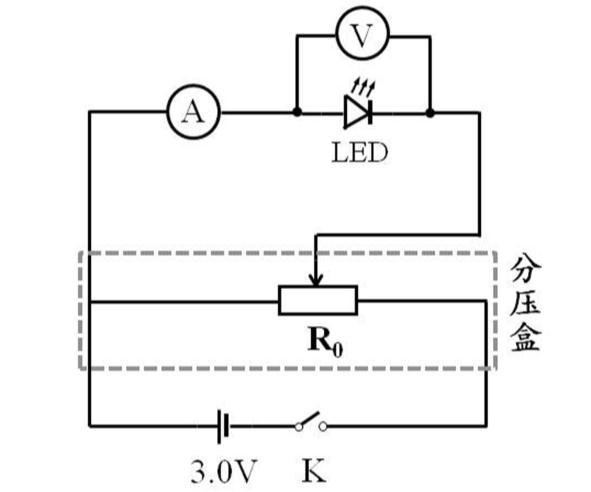
\includegraphics[width=7cm]{fuantexing.png}
    \end{figure}

    \emph{\\[0.02cm]\zihao{-4}2.测量LED光强与工作电流的关系} 

    在$0mA$至$100mA$内,测量绿色 LED 的相对光强与电流的关系,绘制绿色 LED 的$U-I$特
    性曲线,给出近似函数关系。
    \begin{figure}[ht]
        \centering 
        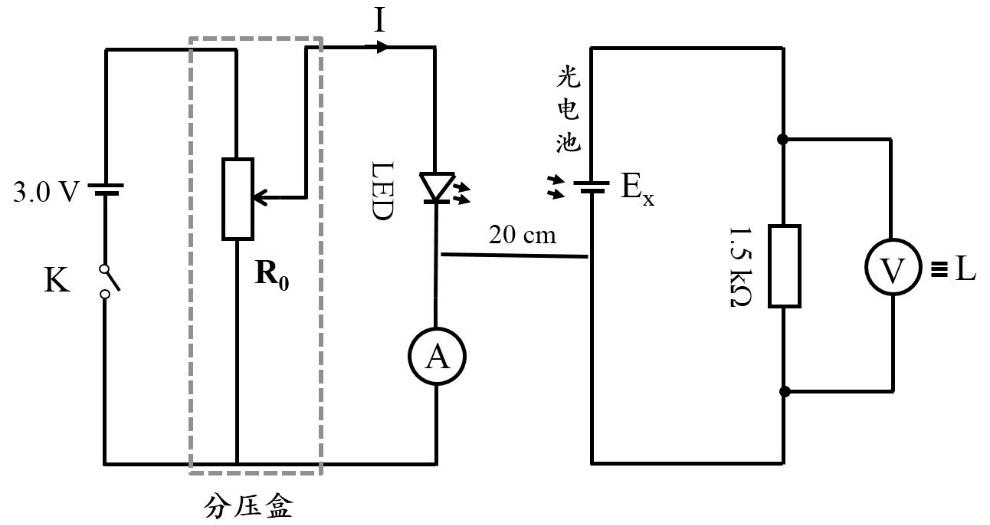
\includegraphics[width=7cm]{faguagnqiangdu.png}
    \end{figure}

    \emph{\\[0.02cm]\zihao{-4}3.加法混色实验}

    将红、绿、蓝 LED 光源作为 RGB 三基色,相加混合法配出指定色卡的颜色。
    按下图接线,调节分压盒,分别采用两个或三个 LED,在$0$至$100mA$内,配出标准色卡的黄色、青色、
    紫色和白色。将光电池放置于白屏处,记录 LED 配色光相对光强与合色光相对光强 ,给出基色的光强比。
    \begin{figure}[ht]
        \centering 
        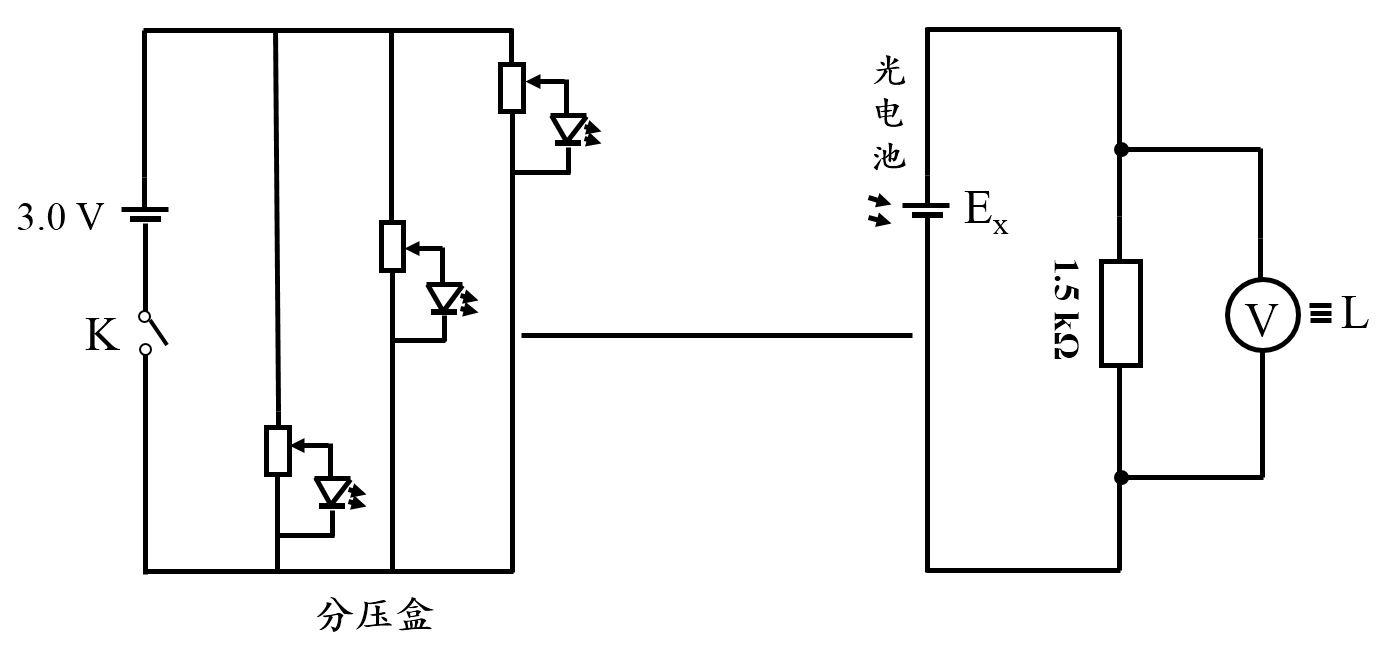
\includegraphics[width=7cm]{peise2.png}
    \end{figure}

    \section{实验记录}
    原始数据附于报告最后

    \section{数据处理}
    \begin{center}
    \emph{\zihao{-4}1.三种单色光的伏安特性曲线}
    \end{center}

    以LED灯工作电流(mA)为X轴、工作电压(V)为Y轴,做出三种单色LED的伏安特性曲线,再选取曲线的线性部分做拟合如下:
    \begin{figure}[ht]
        \centering 
        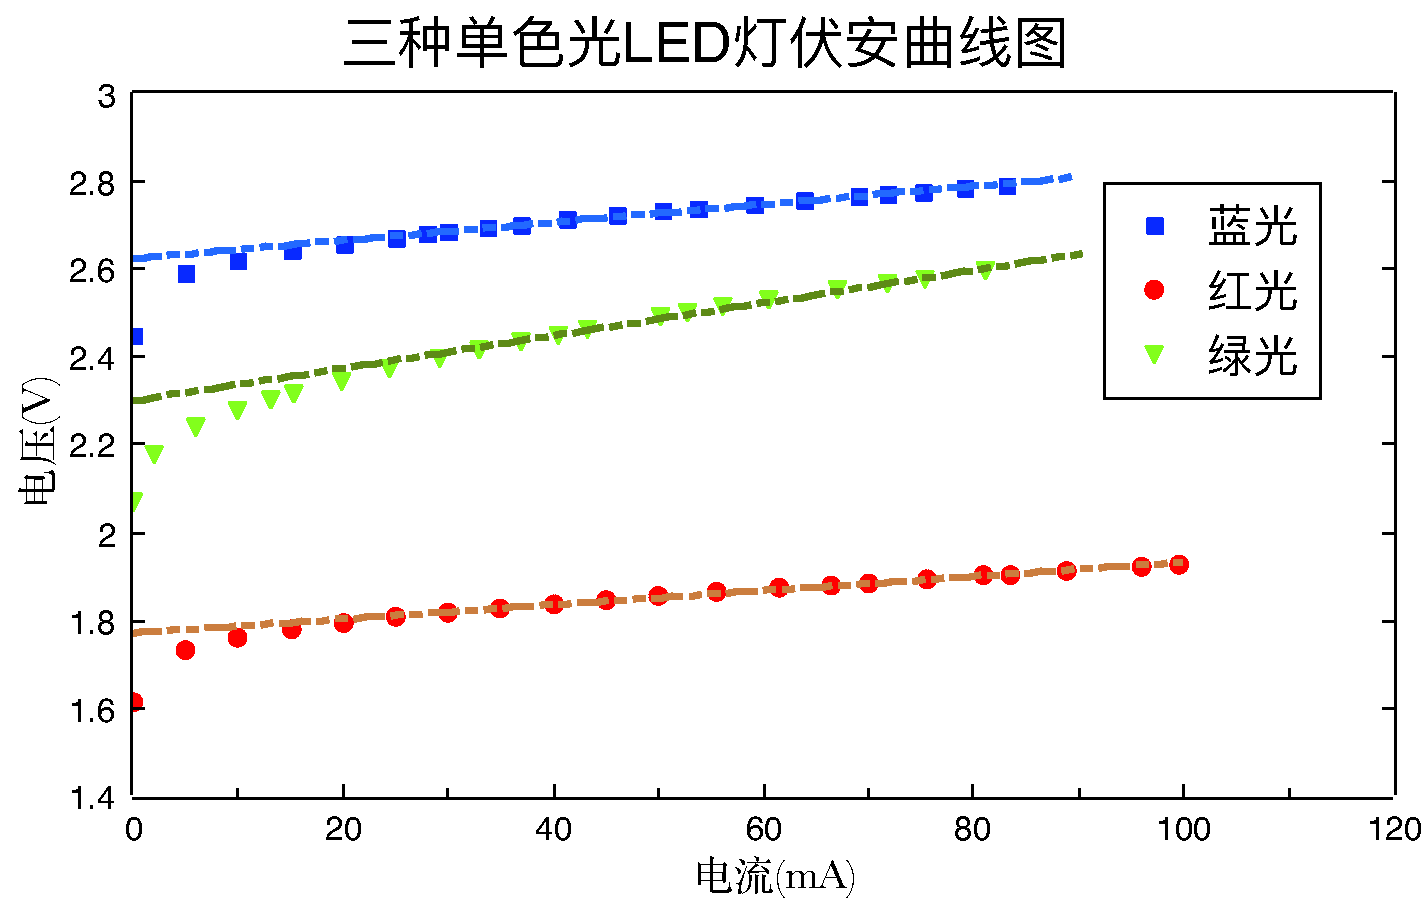
\includegraphics[width=12cm]{三种灯.pdf}
    \end{figure}

    \emph{蓝光拟合曲线:}
    \begin{equation*}
        y=0.002x+2.625
    \end{equation*}
    \begin{equation*}
        R=0.9951
    \end{equation*}

    \emph{绿光拟合曲线:}
    \begin{equation*}
        y=0.0037x+2.3005
    \end{equation*}
    \begin{equation*}
        R=0.9958
    \end{equation*}

    \emph{红光拟合曲线:}
    \begin{equation*}
        y=0.0016x+1.7714
    \end{equation*}
    \begin{equation*}
        R=0.9912
    \end{equation*}

    图像中选择线性拟合的数据点基本落在拟合直线上,且三种拟合直线的$R^2$均大于0.99,表明有很强的线性相关性,拟合可信度高。

    \begin{center}
    \emph{\zihao{-4}2.三种LED灯的发光波长}
    \end{center}

    实验数据自电流恰好为0处开始测量,从图中可以得知蓝光LED、绿光LED、红光LED的导通阈值电压分别为
    2.625V、2.3005V、1.7714V,计算如下:
    
    \emph{蓝色LED灯:}
    \begin{equation*}
        E_{blue}=U_{blue}*e=2.625*1=2.625(ev)
    \end{equation*}
    \begin{equation*}
        \lambda =\frac{1240}{E_g}=\frac{1240}{2.625}=472.380(nm)
    \end{equation*}

    \emph{绿色LED灯:}
    \begin{equation*}
        E_{green}=U_{green}*e=2.070*1=2.070(ev)
    \end{equation*}
    \begin{equation*}
        \lambda =\frac{1240}{E_g}=\frac{1240}{2.070}=599.034(nm)
    \end{equation*}

    \emph{红色LED灯:}
    \begin{equation*}
        E_{red}=U_{red}*e=1.6122*1=1.6122(ev)
    \end{equation*}
    \begin{equation*}
        \lambda =\frac{1240}{E_g}=\frac{1240}{1.6122}=769.135(nm)
    \end{equation*}

    \begin{center}
    \emph{\zihao{-4}3.绿色LED灯光强与工作电流关系}
    \end{center}

    以绿色LED灯工作电流(mA)为X轴、光电池在$1.5k\varOmega $负载下的输出电压为Y轴,分别进行完全拟合(图1)、部分拟合(图2)、二次多项式拟合(图3)以及自然对数拟合(图4),作图如下:
    \begin{figure}[ht]
        \centering 
        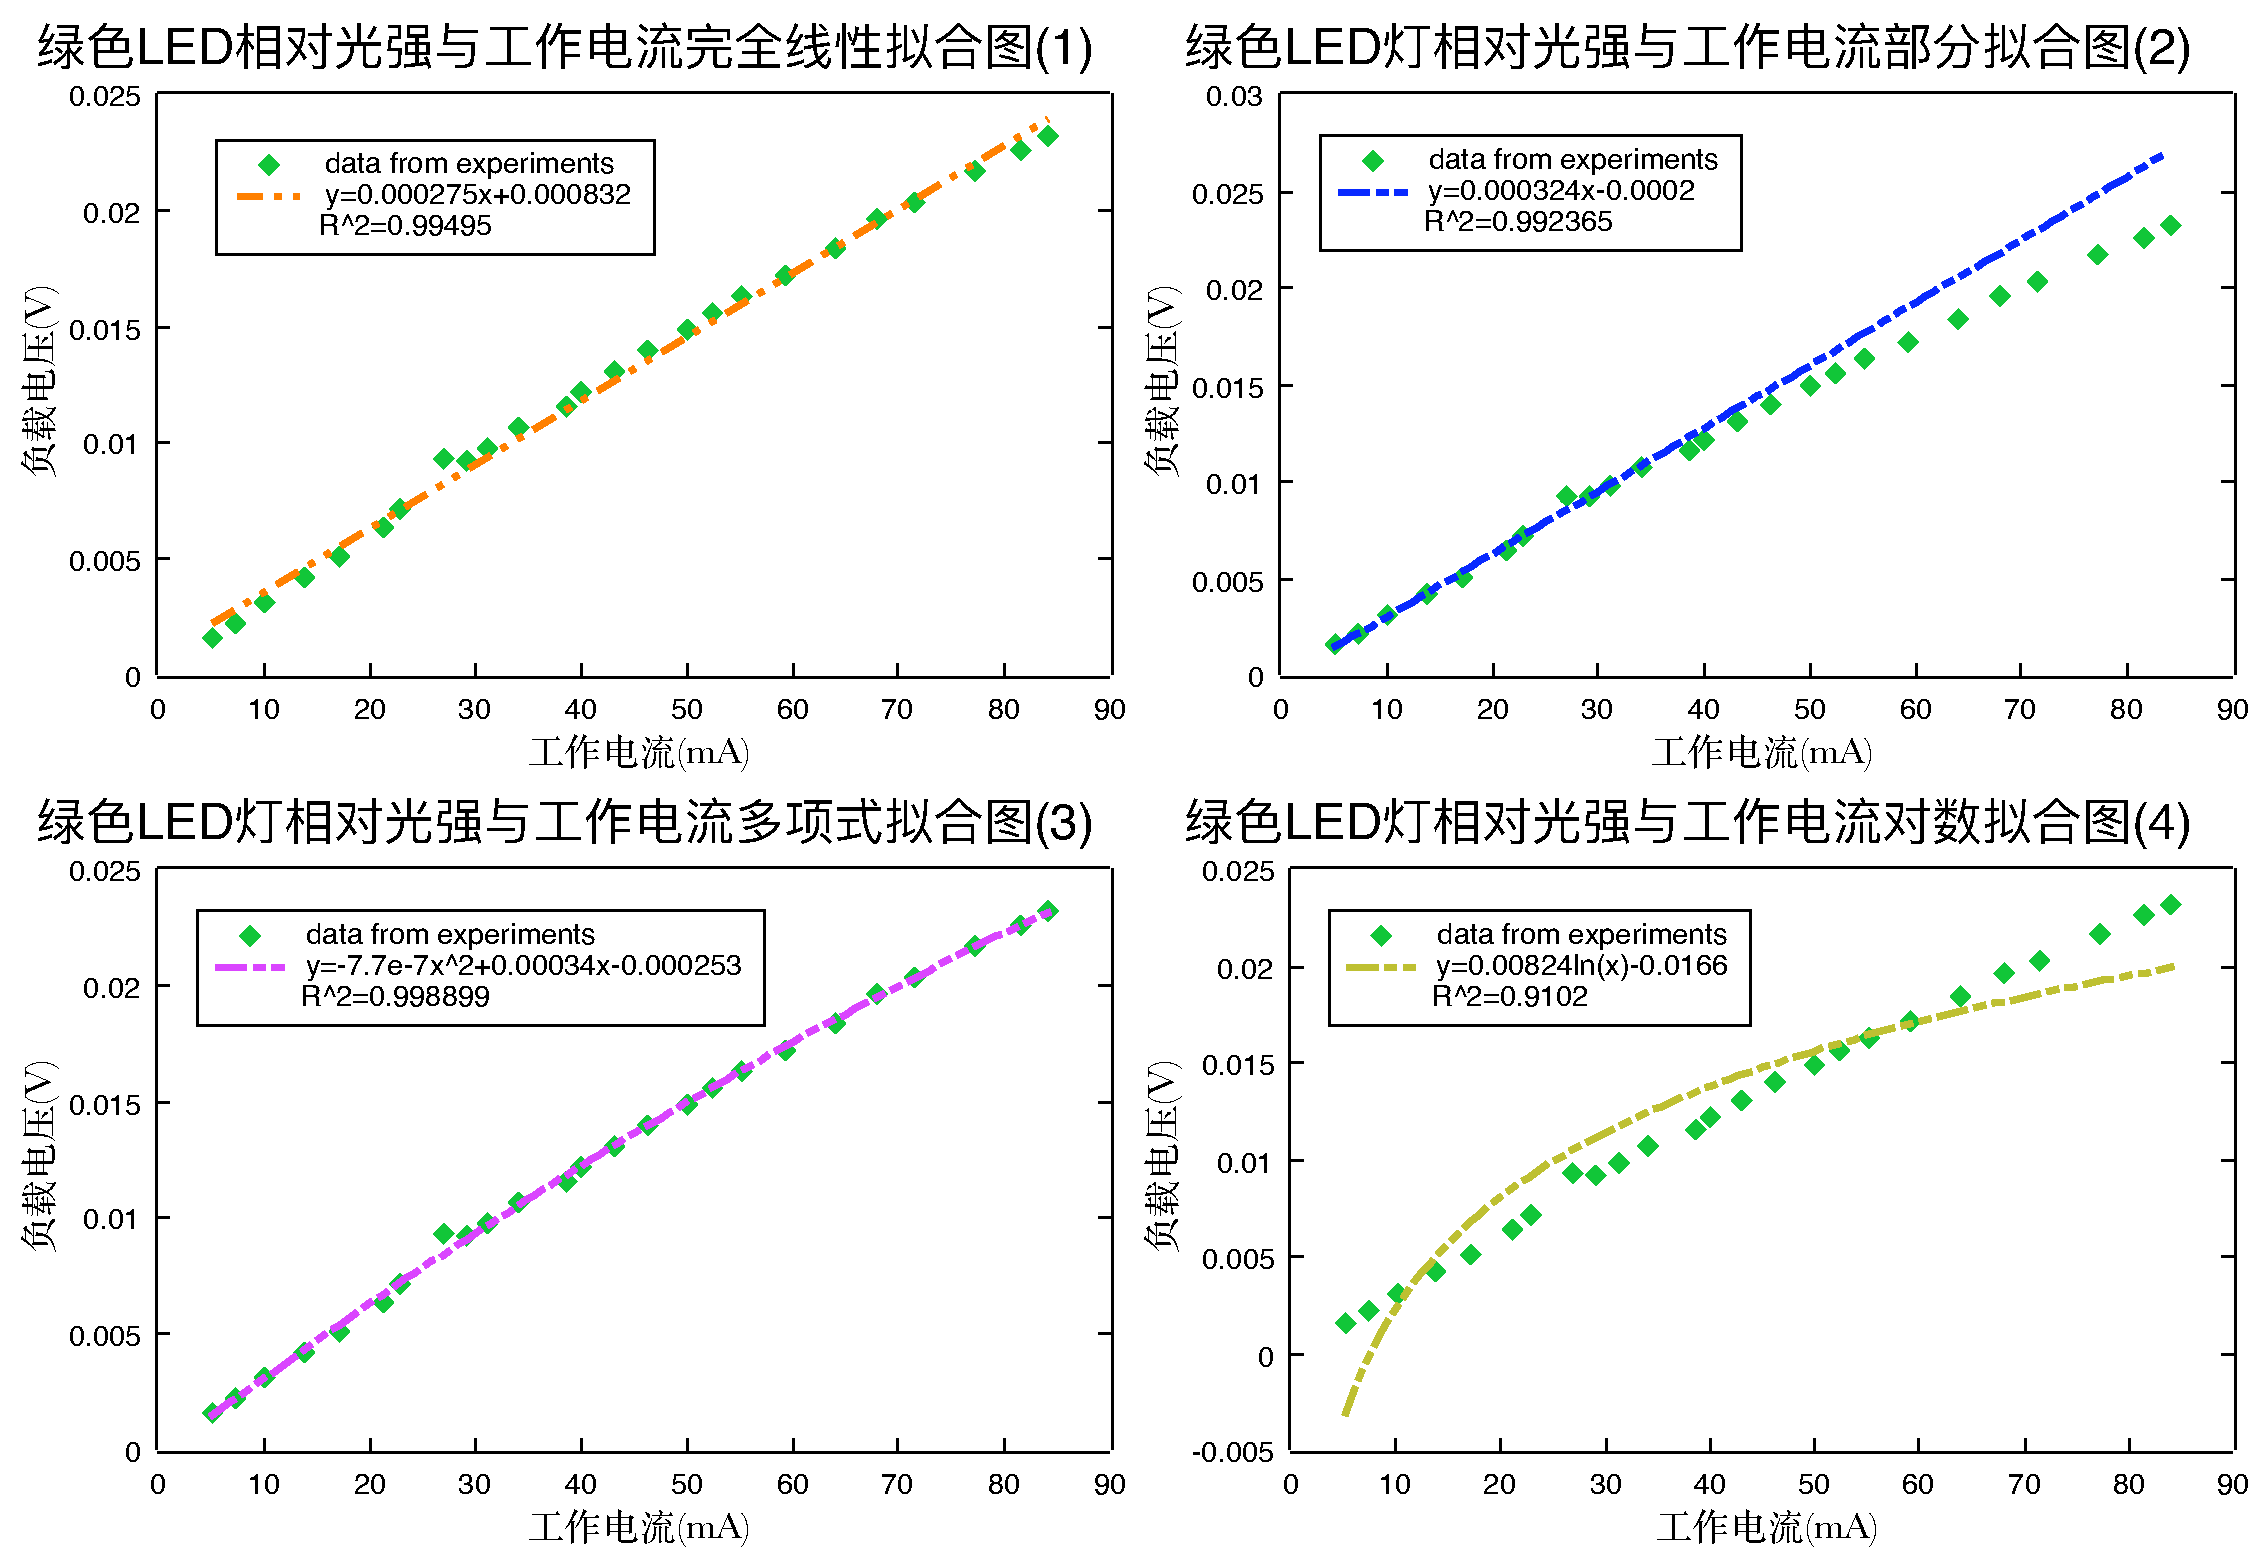
\includegraphics[width=16cm]{zhengque.pdf}
    \end{figure}

    图(1)使用了测得的全部数据作线性拟合,从图中可以看出,绿色数据点有比较明显的分区分布:30mA之前的数据基本分布在拟合曲线下侧、30mA-60mA的数据点基本分布在拟合曲线上侧、60-90mA数据点
    又分布在拟合曲线下侧。这表明使用线性拟合全部的数据是不合适的,真正的U-I关系有较为明显的弯曲倾向。

    观察到0-35mA的数据点基本落在一条直线附近,取之作新的拟合曲线如图(2).可以看到数据点弯曲的趋势较为明显,于是分别使用二次多项式与自然对数拟合数据点,作出图(3)与图(4)。

    从图中可以看到,虽然对数图像是上凸函数,然而曲率过大,$R^2$是这四种拟合中最小的,显然不是最佳拟合。而使用二次多项式的拟合曲线图像中,所有的数据点都分布在拟合曲线两侧,且$R^2$达到0.998899
    ,是这四幅图中拟合范围最广、拟合效果最好的函数。如果认为这就是最佳拟合曲线,有一定的科学性。

    \emph{\zihao{-4}故近似函数关系为:}
    \begin{equation*}
        y=-7.7*10^{-7}x^2+0.00034x-0.000253
    \end{equation*}

    \begin{center}
        \emph{\zihao{-4}4.加法混色实验}
    \end{center}

    \emph{黄色:}

    黄光由红色与绿色混合而成,从数据可以看出,绿色成分与红色成分的比值约为$1:2$,总光强大约是两种单色光光强之和,符合配色方程。

    \emph{青色:}

    青光由绿光和蓝光混合而成,计算可知,绿色成分与蓝色成分的比值约为$7:8$,然而总光强明显小于两种单色光光强之和。

    \emph{紫色:}

    紫光由红光与蓝光混合而成,从数据中可以得知红色成分与蓝色成分的比值约为$5:7$,且总光强符合单色光光强之和。

    \emph{白色:}

    白光由红绿蓝三色光混合而成,计算可知红:绿:蓝约为$8:9:10$,结果符合配色方程。

    \section{误差分析}

    \emph{\zihao{-4}1.发光波长实验:}

    查询资料得知,三基色标准波长波长分别为 700nm、546.1nm、435.8nm,而本次实验计算得到的三种颜色的波长均偏大,分析有以下原因:

    如果实验使用的LED灯发出的光是标准波长,那么波长偏大的直接原因是$E_g$偏小,由于$E_g$与阈值电压$U_D$有正比关系,则$U_D$偏小。而$U_D$是
    线性拟合曲线在U轴上的截距,如果截距偏小,说明直线的斜率偏大,所以一个可能的原因,
    是一些一些小电流对应的数据点不在线性区间,却被选入参与拟合直线的计算,导致拟合斜率偏大

    也有可能是因为实验中使用的三色LED灯发光并不是标准波长。

    \emph{\zihao{-4}2.加法混色实验:}

    如果实验使用的三色LED灯发的光不是标准波长,则可以解释为什么白光的实验配比与在标准基色光下比例 1.0000:4.5907:
    0.0601 有所差异:如果实验使用的的红光波长远小于$700nm$,则红光的确应当占据更大的比例。
    
    然而实验的与标准基色光的比例差异实在太大,由于配色实验有较强的主观性,每个人视锥细胞的数量和构造都有所差异;加之
    做实验时的昏暗环境,以及配了很久颜色已经分不清这是什么颜色的疲劳状态,很容易导致较大的实验误差误差。


    \section{提出改进}
    配色实验使用的颜色卡片需要一些改进。
    
    既然单色光只要比例相同配出的颜色就相同,
    而且暗环境下人盯着较强光亮区域容易引发视觉疲劳,以致分不清这究竟有没有真的配上卡片上的底色,
    那么不妨提高色卡的颜色饱和度,能让同学们更清楚分辨光色与底色的差异。


    \section{思考题}
    
    \emph{\\[0.02cm]\zihao{-4}1.LED的发光原理是什么?LED的发光强度及颜色与哪些因素有关?}

    LED灯由PN结为核心构件,当正向电压加在发光二极管时,电子由 N 区注入 P 区,空穴由 P 区注入 N 区,从而结区出现不平
衡状态,这些注入的的电子与空穴在 PN 结区发生复合,释放能量,发射光子。此外,如果一些电子被无辐射中心俘
获,能量以热能形式散发,称为非辐射复合。辐射复合相对于非辐射复合比例越大,光量子效率越高。实验证明,发射光子的能量与材料能隙有关,而根据电磁波的能量转换公式:
\begin{equation}
    E=h\nu 
\end{equation}
可知波长与空穴-电子复合释放的能量的关系。

    \emph{\\[0.02cm]\zihao{-4}2.甲光 R:G:B 为 1:2:3;乙光 R:G:B 为 2:4:6,甲光和乙光有什么区别?}

    颜色上相同,强度上甲光是乙光的一半.

    \emph{\\[0.02cm]\zihao{-4}3.色光混合及色料混合的基本规律?色料三原色的补色分别是什么颜色?}

    色光混合遵循加法混色原理,一种基色光中加入另一种基色光,可以合成第三种色彩,色光越多,色彩亮度越强。
    
    根据三基色理论,自然界任意一种光都能被分解成红绿蓝三色光的线性组合,红绿蓝三色是配色空间的一组基,维数为3.

    色料混合遵循减法混色原理,颜色能吸收入射光中的部分成分,其他成分被反射,形成该颜料独特的色彩。

    一种颜料中加入另一种颜料可以合成第三种颜色的颜料,颜料越多,颜色越暗。

    颜料的三原色分别为品红、黄、青。分别的补色为绿色、紫色、橙色。
    \nocite{dawushiyan}
    \nocite{shiyanjiaocheng}
    \nocite{jiangyi}
    \bibliography{math}

\end{document}
